\documentclass[aps,prd,twocolumn,nofootinbib]{revtex4-1}
\usepackage{amsmath}
\usepackage{graphicx}
\usepackage{subfig}
\usepackage{epsfig}
\usepackage{listings}
\usepackage[hidelinks,hyperfootnotes=false,bookmarks=false]{hyperref}
\usepackage[colorinlistoftodos]{todonotes}
\usepackage{verbatim}
\usepackage{float}
\begin{document}
\title{A Survey of Sterile Neutrinos}
\author{Douglas Davis}
\author{Matthew Epland}
\author{Justin Raybern}
\author{Pingchuan Zhao}
\affiliation{Department of Physics, Duke University, Durham, NC 27707, USA}
\date{\today}
\begin{abstract}
Neutrinos are light, weakly interacting, left-handed leptons in the Standard Model of particle physics. The discovery of neutrino oscillations (suggesting neutrinos actually have mass) has led to a fruitful time in neutrino research. Oscillation experiments measure the oscillation parameters $\Delta m^2$ and $\sin^2 2\theta$, which are the mass splittings of neutrino mass eigenstates and the mixing angles of a unitary transformaton matrix that governs the oscillation probabilities. Experiments have measured these parameters, and some results suggest the existence of the expected three weakly interacting neutrinos, but also the possibility of more neutrinos which are not weakly interacting, and are therefore given the name ``sterile'' neutrino. We summarize the theory and experimental evidence in the sterile neutrino sector.
\end{abstract}\maketitle
\section{Introduction}
The Standard Model of Particle Physics continues to succeed wonderfully in making predictions in nature.  The discovery of the Higg's Boson is just one example of the predictive power of the model.  There are places in nature, however, where the Standard Model fails - the fact that neutrinos have mass, which is confirmed by flavor oscillations, is completely outside the model.  The smallness of the neutrino mass cannot be explained definitively by theory either.  And even more interestingly, neutrinos seem to only come as left-handed particles.

In this work we lay out some of basic Standard Model theory concerning neutrinos.  We then describe oscillations and the significance of that behavior.  We then explain sterile neutrinos - neutrinos that do not interact via the weak force, and how the see-saw model of neutrino mass can simultaneously explain light, left-handed neutrinos.  We discuss some of the contested experimental evidence for sterile neutrinos and future experimental work in the field.
\section{Theory}
\label{sec:theory}
\subsection{Standard Model, and Beyond, Neutrinos}
A neutrino is an electrically neutral, weakly interacting elementary particle with half integer spin. There are three generations of leptons and their corresponding neutrino: electron \& electron-neutrino, muon \& muon-neutrino, and tau \& tau-neutrino. Neutrinos were first postulated as products in beta decay. From the experiment of radioactive decay, the outgoing electron energy varies; therefore it is not a 2-body decay, but actually a 3-body decay. Pauli first called that small, neutral charge particle neutrino.

In the Standard Model, there are three generations of neutrinos, and the Lagrangian has no neutrino mass term. Also, neutrinos and anti-neutrinos are distinct, separated by helicity. From experiment measurements, neutrinos always have left helicity and anti-neutrinos with right helicity. Neutrinos couple ony with the $W$ and the $Z$ bosons in this model~\cite{ping1}.

Although the Standard Model is exceedingly successful in explaining the interactions of fundamental particles, it can not be the ultimate theory, since it does not give explanations for gravity, dark matter, and now known neutrino mass, which is evident from neutrino oscillations. In the 1960s, the solar neutrino experiment first indicated that there is a change of flavor when neutrinos traveling. This is also the first evidence that shows neutrinos have mass (see section~\ref{sec:oscillate} for discussion of oscillations and mass). By using the detector Kamiokande and later the upgraded version, Super Kamiokande, they observe the flavor changes not only from solar neutrinos but also long-baseline reactor neutrinos and atmospheric neutrinos.

Starting in the late 1960s, there is a discrepancy using Standard Model to give explanations to neutrinos arriving from the sun~\cite{ping2}. The observed electron neutrinos are only between one third to one half of what Standard Model predicts. This problem remains unsolved until almost 30 years later as the observation of neutrino oscillation, which give a perfect explanation on solar neutrino problem. Since the neutrinos are changing flavors when traveling, the fraction of electron has changed to other flavors, and the fraction can be calculated from the mixing angles of oscillations. The mixing angles now have all been experimentally determined, with the last one $\theta_{13}$ found in 2012 in Daya Bay experiment~\cite{ping3}. However, the mixing angles and oscillation experiment only gives the relative mass between different flavors of neutrinos, this can not give the absolute mass of neutrinos. Hence the neutrino mass is crucial problem to understand nowadays. Neutrinos may be Majorana particles which is that they are their own antiparticles. If this is true, then not only the absolute mass of neutrinos can be observed, but also it explains why after the universe evolves, the matter dominates over anti-matter~\cite{ping4}.

\subsection{Oscillations}
\label{sec:oscillate}
Neutrino oscillations were theorized by Bruno Pontecorvo In the 1950's, when he believed neutrinos would oscillate between $\nu$ and $\overline{\nu}$ states similar to the mixing of neutral kaons $K^0$ and $\overline{K}^0$~\cite{ponte}. The theory that an electron neutrino could oscillate to a muon neutrino was first considered by Maki, Nakagawa, and Sakata~\cite{MNS}.

In neutrino oscillation theory, neutrino mass eigenstates $|\nu_j\rangle$ are expressed as linear superposition of the flavor states, $|\nu_{\alpha}\rangle$, where $\alpha = e,\mu,\tau$:
\begin{equation}
  \left|\nu_j\right\rangle = \sum_{\alpha}U_{\alpha j}\left|\nu_{\alpha}\right\rangle,
  \label{mass=flavor}
\end{equation}
where $U$ is a $3\times3$ unitary matrix called the PMNS (Pontecorvo, Maki, Nakagawa, Sakata) matrix. The matrix can be inverted to write the flavor eigenstates as a superposition of the mass eigenstates:
\begin{equation}
  \left|\nu_{\alpha}\right\rangle = \sum_{j=1}^3U^*_{\alpha j}\left|\nu_{j}\right\rangle.
  \label{flavor=mass}
\end{equation}
Since the mass eigenstates have definite mass, $m_j$, and energy, $E_j$, they can be evolve in time as established by the Schr\"odinger Equation:
\begin{equation}
  \mathcal{H}\left|\nu_j(t)\right\rangle = i\hbar \frac{\partial}{\partial t}\left|\nu_j(t)\right\rangle,
  \label{nu-schro1}
\end{equation}
yielding
\begin{equation}
  \left|\nu_j(t)\right\rangle = e^{-iE_jt}\left|\nu_j\right\rangle,
  \label{nu-schro2}
\end{equation}
where $|\nu_j\rangle = |\nu_j(t=0)\rangle$. Combining with equation \ref{flavor=mass}:
\begin{equation}
  \left|\nu_{\alpha}(t)\right\rangle = \sum_{j=0}^3 U_{\alpha j}^* e^{-iE_jt}\left|\nu_j\right\rangle,
  \label{flavor_whole}
\end{equation}
and now combining equation \ref{flavor_whole} with equation \ref{mass=flavor}:
\begin{equation}
  \left|\nu_{\alpha}(t)\right\rangle = \sum_{\beta=e,\mu,\tau}\sum_{j=0}^3U_{\beta j}U_{\alpha j}^* e^{-iE_jt}\left|\nu_{\beta}\right\rangle.
\end{equation}
The probability that a neutrino of flavor state $\nu_{\alpha}$ will oscillate into $\nu_{\beta}$ is written as:
\begin{eqnarray}
  P(\nu_{\alpha}\rightarrow\nu_{\beta}) &=& |\langle\nu_{\beta}|\nu_{\alpha}\rangle|^2 \nonumber \\
                                        &=& \left|\sum_{j=0}^Ne^{-iE_jt}U_{\beta j}U_{\alpha j}^*\right|^2 \nonumber \\
                                        &=& \sum_{j=1}^3\sum_{k=1}^3U_{\alpha j}^*U_{\alpha k}U_{\beta j}U_{\beta k}^*e^{-i(E_j-E_k)t}.
\end{eqnarray}
In the ultra-relativistic limit (which neutrinos qualify for with $v \approx c$), we can write:
\begin{equation}
  E_i = \sqrt{m_i^2+p^2} \approx p + \frac{m_i^2}{2p} \\
  \label{eq:approx1}
\end{equation}
\begin{equation}
  E_j - E_k \approx p + \frac{m_j^2}{2p} - \left(p + \frac{m_k^2}{2p}\right),
  \label{eq:approx2}
\end{equation}
and using $E \approx p$ (continuing with the ultra-relativistic limit):
\begin{equation}
  E_j - E_k = \frac{m_j^2 - m_k^2}{2E}.
  \label{eq:approx3}
\end{equation}
Now we adopt the relation $\Delta m_{jk}^2 = m_j^2 - m_k^2$, and use $L = ct$, where $c\equiv1$,\footnote{we have been using $\hbar \equiv 1$ as well, adopting natural units for this derivation} to write:
\begin{equation}
  P(\nu_{\alpha}\rightarrow\nu_{\beta}) = \sum_{j=1}^3\sum_{k=1}^3U_{\alpha j}^*U_{\alpha k}U_{\beta j}U_{\beta k}^*e^{-i\Delta m_{jk}^2L/2E}.
\end{equation}
We can now write a complete expression without a complex exponent as:
\begin{widetext}
  \begin{align}
    \begin{split}
      P(\nu_{\alpha}\rightarrow\nu_{\beta}) = \delta_{\alpha\beta} & - 4\sum_{j>k}\Re\left(U_{\alpha j}^*U_{\alpha k}U_{\beta j}U_{\beta k}^*\right)\sin^2\left(\frac{\Delta m_{jk}^2}{4E}L\right) \\
      & + 2\sum_{j>k}\Im\left(U_{\alpha j}^*U_{\alpha k}U_{\beta j}U_{\beta k}^*\right)\sin\left(\frac{\Delta m_{jk}^2}{2E}L\right).
    \end{split}
  \end{align}
\end{widetext}
  We can write the unitary PMNS matrix as~\cite{matrixpara}, where $\delta$ is the neutrino sector $CP$ violating phase:
\begin{widetext}
  \begin{align}
    \begin{split}
      U & =
      \begin{pmatrix}
        U_{e1}    & U_{e2}    & U_{e3}   \\
        U_{\mu1}  & U_{\mu2}  & U_{\mu3} \\
        U_{\tau1} & U_{\tau3} & U_{\tau3}
      \end{pmatrix} \\
      \label{eq:umatrix}
      & = \begin{pmatrix}
        1 & 0 & 0 \\
        0 & c_{23} & s_{23} \\
        0 & -s_{23} & c_{23} \end{pmatrix} \times
      \begin{pmatrix}
        c_{13} & 0 & s_{13}e^{-i\delta} \\
        0      & 1 & 0 \\
        -s_{13}e^{i\delta} & 0 & c_{13} \end{pmatrix} \times
      \begin{pmatrix}
        c_{12} & s_{12} & 0 \\
        -s_{12} & c_{12} & 0 \\
        0 & 0 & 1
      \end{pmatrix} \\
      & = \begin{pmatrix}
        c_{12}c_{13} & s_{12}c_{13} & s_{13}e^{-i\delta} \\
        -s_{12}c_{23} - c_{12}s_{23}s_{13}e^{i\delta} & c_{12}c_{23} - s_{12}s_{23}s_{13}e^{i\delta} & s_{23}c_{13} \\
        s_{12}s_{23} - c_{12}c_{23}s_{13}e^{i\delta} & -c_{12}s_{23} - s_{12}c_{23}s_{13}e^{i\delta} & c_{23}c_{13}
      \end{pmatrix}.
    \end{split}
  \end{align}
\end{widetext}
In a simplified model, for example a two neutrino case, we can write the mixing matrix as:
\begin{equation}
  U = \begin{pmatrix}
    \cos\theta & \sin\theta \\
    -\sin\theta & \cos\theta
  \end{pmatrix}.
\end{equation}
If we consider a two neutrino case consisting of $\nu_{\mu}$'s and $\nu_e$'s, we can write:
\begin{equation}
  \begin{pmatrix}
    \nu_e \\
    \nu_{\mu}
  \end{pmatrix} = \begin{pmatrix}
    \cos\theta & \sin\theta \\
    -\sin\theta & \cos\theta
  \end{pmatrix}
  \begin{pmatrix}
    \nu_1 \\
    \nu_2
  \end{pmatrix}
\end{equation}
\begin{eqnarray}
  \left|\nu_{\mu}(t)\right\rangle &=& -\sin\theta e^{-iE_1t}\left|\nu_1\right\rangle+\cos\theta e^{-iE_2t}\left|\nu_2\right\rangle \\
  \left|\nu_e\right\rangle &=& \cos\theta\left|\nu_1\right\rangle+\sin\theta\left|\nu_2\right\rangle
\end{eqnarray}
Utilizing equations \ref{eq:approx1}, \ref{eq:approx2}, \ref{eq:approx3} and adopting $L=t$ once again:
\begin{equation}
  P(\nu_{\mu}\rightarrow\nu_e) = |\langle \nu_e | \nu_{\mu}(t)\rangle|^2 = \sin^2 2\theta \sin^2\left(\frac{\Delta m^2 L}{4E}\right).
\end{equation}
Conversion from natural units to units common to the laboratory, we arrive at a probability equation of the form:
\begin{equation}
  P(\nu_{\mu}\rightarrow\nu_e) = \sin^22\theta\sin^2\left(\frac{1.27\Delta m^2 \left[\text{eV}^2\right] L [\text{km}]}{E[\text{GeV}]}\right).
  \label{eq:osc}
\end{equation}
Naturally, the probability of survival is defined as:
\begin{equation}
  P(\nu_{\mu}\rightarrow\nu_{\mu}) = 1-\sin^22\theta\sin^2\left(\frac{1.27\Delta m^2 \left[\text{eV}^2\right] L [\text{km}]}{E[\text{GeV}]}\right).
  \label{eq:surv}
\end{equation}
Oscillation and survival probabilities for $\nu_\mu\rightarrow\nu_e$ are shown in Figure~\ref{fig:probs}.
\begin{figure}[H]
  \centering
  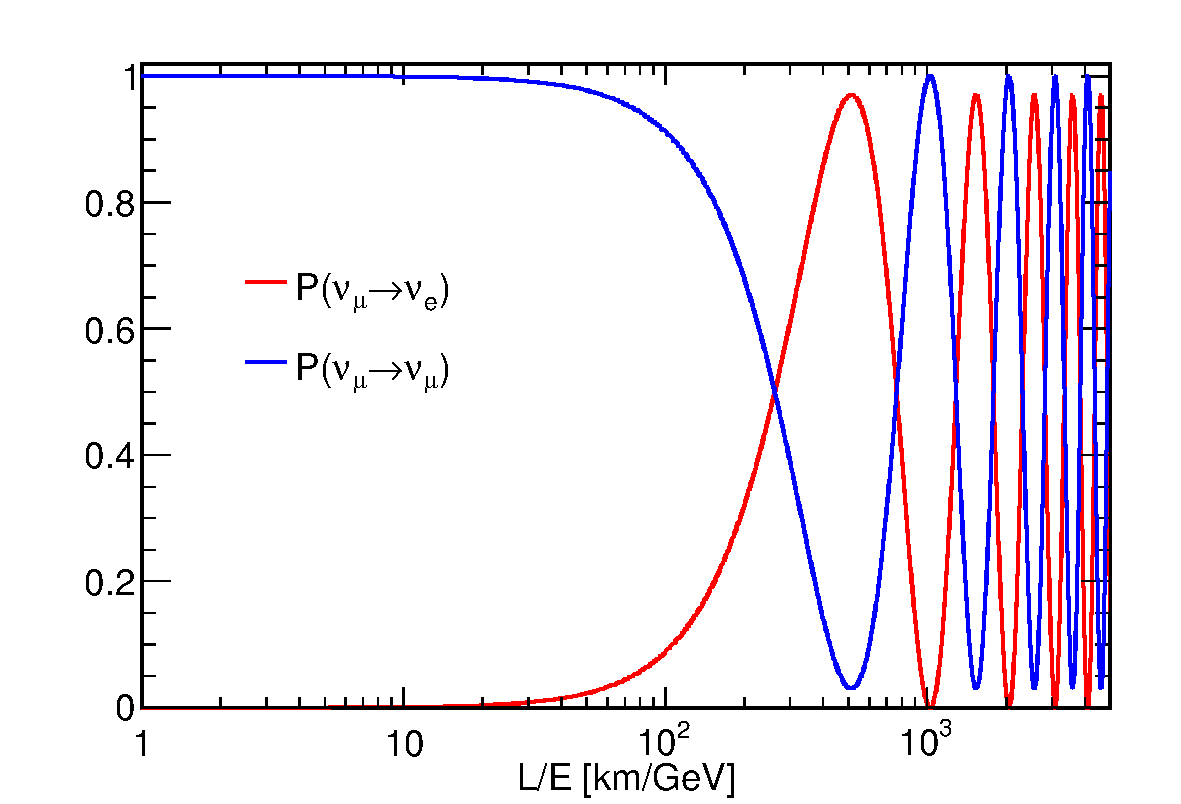
\includegraphics[width=1\linewidth]{../figures/oscillation_prob.pdf}
  \caption{Oscillation and survival probabilities for the two neutrino state with an initial $\nu_{\mu}$. The values for $\Delta m^2$ and $\sin^22\theta$ ($2.41\times 10^{-3}$ eV$^2$ and 0.97, respectively) are taken from 2013 MINOS result (PRL, 110, 251801)}
  \label{fig:probs}
\end{figure}
\subsection{See-Saw Neutrinos}
The See-Saw method is the most common way of explaining the possible existence of sterile neutrinos.  The fact that there are no right-handed neutrinos, despite there being both left- and right-handed leptons, leaves theorists unsatisfied. Experiment confirms the lack of right-handed neutrinos.  The small masses of the neutrinos is also unsettling. This can be reconciled by introducing right-handed terms in the neutrino Lagrangian~\cite{justin1}. The Lagrangian for a neutrino should include a mass term.  The idea of sterile neutrinos arises from the addition of some nonzero right-handed component in the Lagrangian. This is seen in
\begin{align}
  \begin{split}
  \begin{pmatrix}
    \overline{\nu} & \overline{N}
  \end{pmatrix}
  \begin{pmatrix}
    0 & m_D \\ m_D & M
  \end{pmatrix}
  \begin{pmatrix}
    \nu \\ N
  \end{pmatrix},
  \end{split}
\end{align}
where $\nu$ and $N$ are the left- and right-handed neutrino components, respectively. The Dirac mass is given by $m_D$ and the Majorana mass is given my $M$. It is easy to show that the eigenvalues of this matrix, if $m_D \ll M$, are $m_D^2/M$ and $M$ with the approximate eigenvectors associated with the left- and right- handed neutrinos. This means that we have the normal neutrino eigenstate and a sterile neutrino eigenstate. One can see that as $M$ increases or decreases $m_D^2/M$ does the opposite -- thus the name ``see-saw.'' See Figure~\ref{fig:seesaw}.
\begin{figure}[H]
  \centering
  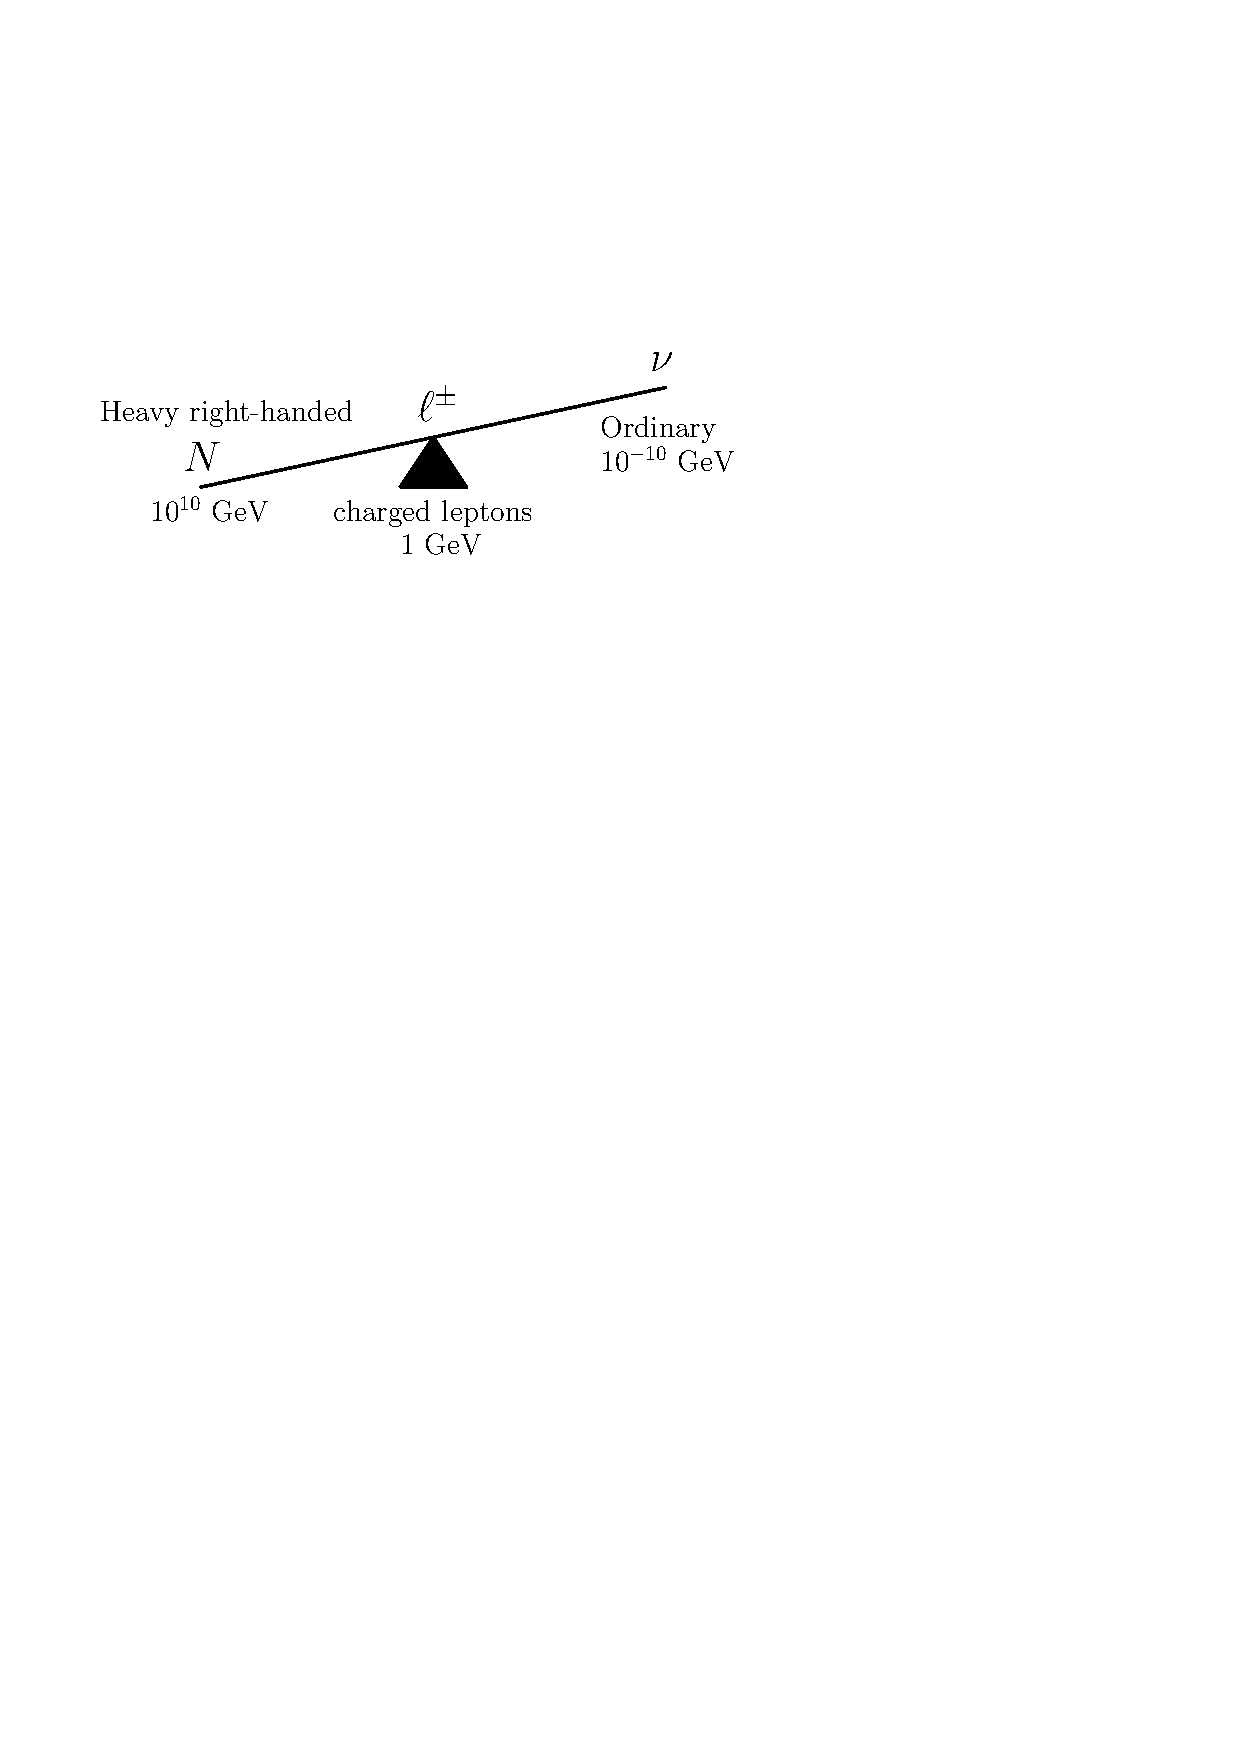
\includegraphics[width=.84\linewidth]{../figures/seesaw.pdf}
  \caption{An illustration of the see-saw mechanism with left handed and right handed neutrino masses}
  \label{fig:seesaw}
\end{figure}

There are different see-saw models associated with the introduction of isospin singlets, scalar triplets, and fermion triplets for types I, II, and III respectively.  The Type I See-Saw model is by far the most popular with theorists.  It suffers from requiring an incredibly large majorana mass around $10^{13}$ GeV making it untestable in current particle accelerators~\cite{justin2}. Type II models also rely on quite large Majorana masses. Type III models have the best chance at experimental verification but are the least phenomenologically satisfying and are thus the least popular.

\section{Previous Experimental Efforts}
There exists considerable experimental evidence for the existence of a fourth neutrino at energy scales in the eV range. The sources for evidence include the short baseline neutrino oscillation experiments LSND (Liquid Scintillator Neutrino Detector) at Los Alamos~\cite{LSND}, and MiniBooNE (Mini Booster Neutrino Experiment) at Fermilab~\cite{mini1,mini2}. There is also the reactor neutrino anomaly~\cite{reactor_anom1}, and also in the radioactive source calibrations for the solar neutrino experiments GALLEX~\cite{gallex1,gallex2} and SAGE~\cite{sage1,sage2}.
\subsection{LSND}
The LSND experiment was developed to search for $\overline{\nu}_\mu \rightarrow \overline{\nu}_e$ oscillations. The source of $\overline{\nu}_\mu$ was the decay at rest (DAR) of $\mu^+$. LSND used a proton beam on a target to produce pions. The decay chain was as follows:
\begin{align}
  \begin{split}
    \pi^+ &\rightarrow \mu^+  \nu_\mu, \\
    \mu^+ &\rightarrow e^+  \nu_e  \overline{\nu}_\mu.
  \end{split}
\end{align}
The $\overline{\nu}_e$ events were detected through the interaction:
\begin{align}
  \overline{\nu}_e  p \rightarrow e^+ n,
\end{align}
inside of a large Cherenkov detector filled with liquid scintillator, utilizing 1280 phototubes. Figure~\ref{fig:lsnd_miniboone}L shows the excess of $\overline{\nu}_e$ events observed by LSND. The observation was $87.9\pm 22.4\pm6$ events over expected background. Their final result claimed the existence of $\overline{\nu}_\mu\rightarrow\overline{\nu}_e$ oscillations at $\Delta m^2 \sim 1\text{ eV}$ with 3.8$\sigma$. This is in heavy conflict with the existing three light flavor neutrino model supported by atmospheric and solar neutrino oscillation experiments, as well as measurements at LEP predicting $N=2.984\pm0.0082$ for weakly interacting neutrino flavors. Therefore, at least one ``sterile'' neutrino is required.
\begin{figure*}
  \centering
  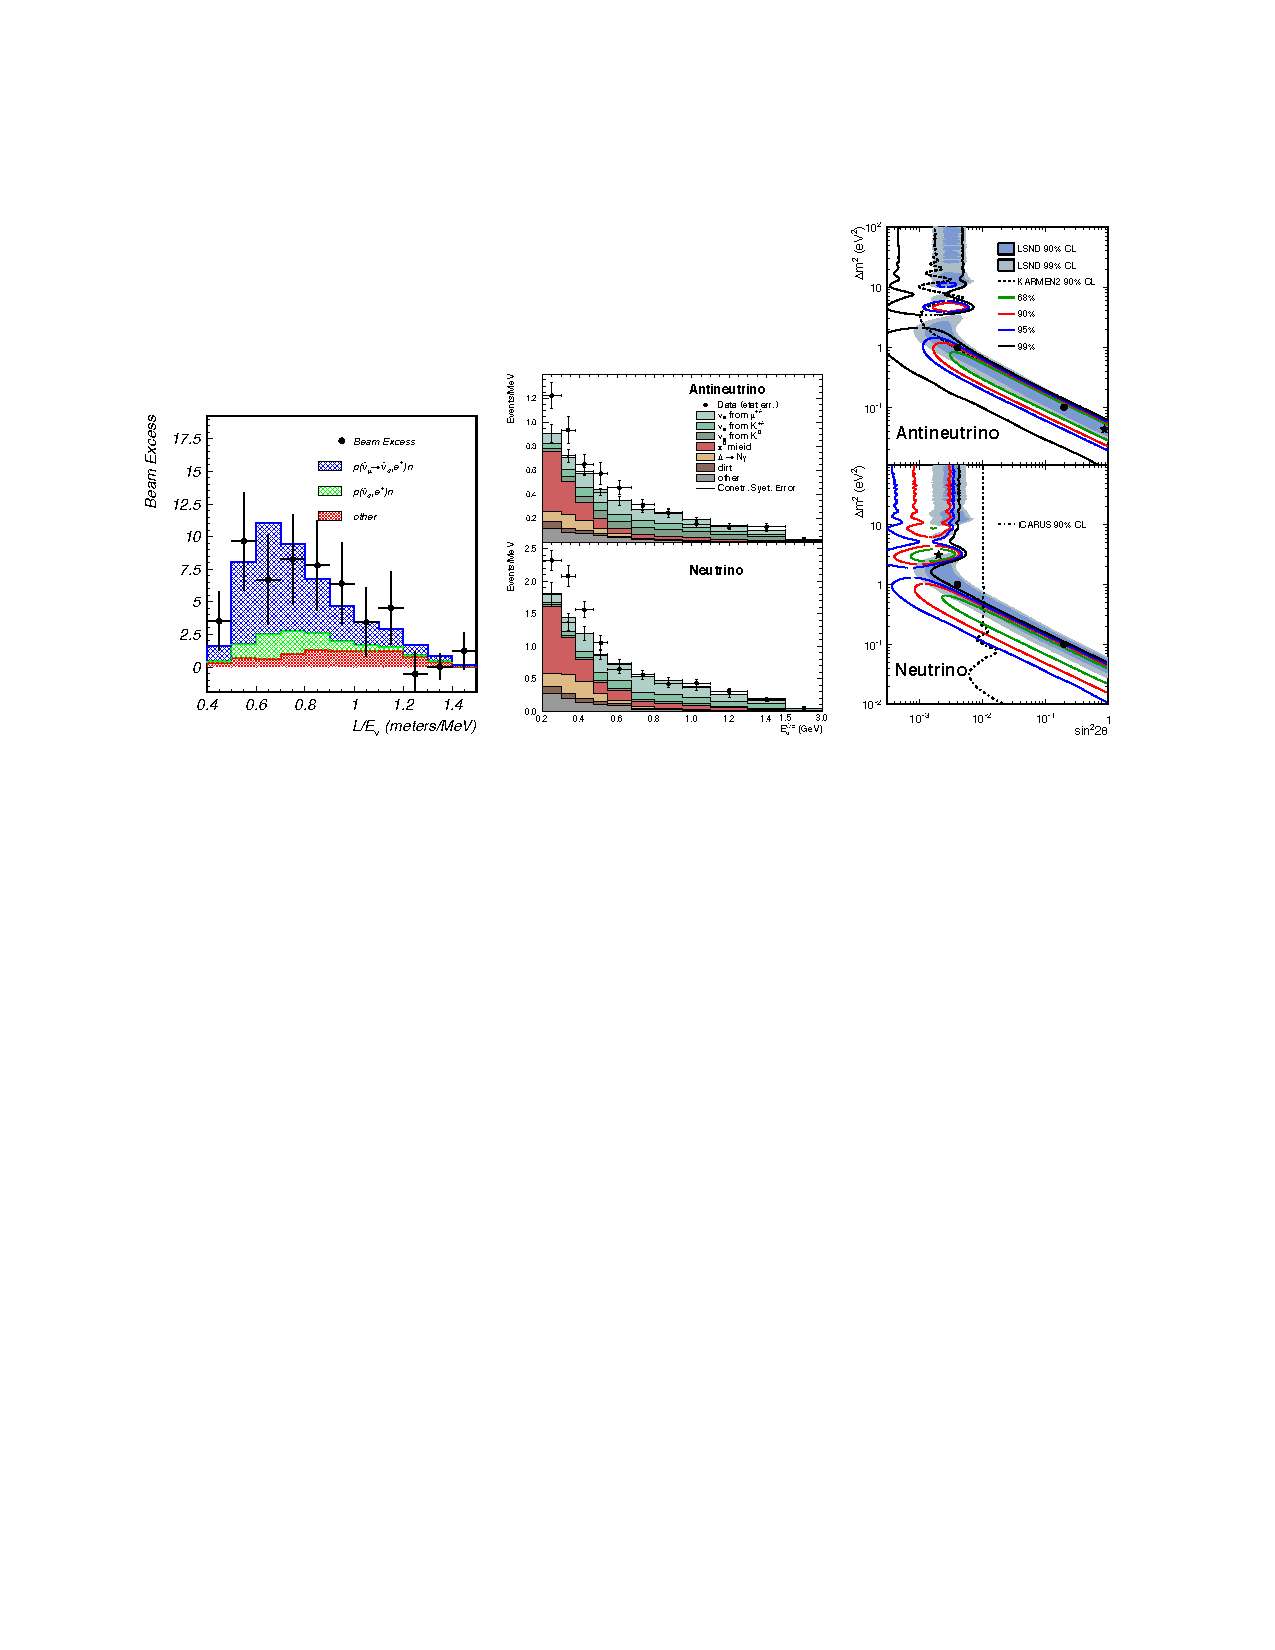
\includegraphics[width=1\textwidth]{../figures/lsnd_miniboone.pdf}
  \caption{(L) From the LSND Experiment~\cite{LSND}. The expected number of events is represented by the red and green histograms, the blue histogram agrees with the data and models $\overline{\nu}_{\mu}\rightarrow \overline{\nu}_e$ oscillation. (C) The MiniBooNE electron event excess in neutrino and anti-neutrino sector~\cite{mini2}. (R) The MiniBooNE allowed regions in neutrino and anti neutrino mode, for a 2 neutrino model. Black stars represent the MiniBooNE best fit points for $\Delta m^2$ and $\sin^22\theta$~\cite{mini2}.}
  \label{fig:lsnd_miniboone}
\end{figure*}
\subsection{MiniBooNE}
The MiniBooNE experiment was developed to answer the LSND anomaly. The MiniBooNE detector also used Cherenkov radiation with photomultiplier tubes as their tool for detecting neutrino interactions. The Booster neutrino beam at Fermilab was used to create a $\nu_\mu$ or $\overline{\nu}_\mu$ beam. Protons were accelerated to 8 GeV by the Booster accelerator and were then steered to a beryillium target where a magnetic focusing horn steered pions from the proton on target collisions down the beam line towards the detector; the pions would decay into muons and muon neutrinos between the horn and the detector. Changing the magnetic focusing horn mode allowed for a beam of mostly $\nu_\mu$ or mostly $\overline{\nu}_\mu$ (neutrino or anti neutrino modes). In neutrino mode $\pi^+$ were steered towards the detector, while $\pi^-$ were steered away; and the reverse for anti neutrino mode. This is to utilize the decays:
\begin{align}
  \begin{split}
    \pi^+ &\rightarrow \mu^+\nu_\mu \\
    \pi^- &\rightarrow \mu^-\overline{\nu}_\mu  
  \end{split}
\end{align}
The full dataset from MiniBooNE was consistent with the LSND $\overline{\nu}_e$ excess, and therefore the sterile neutrino hypothesis survived. Figures~\ref{fig:lsnd_miniboone}C and \ref{fig:lsnd_miniboone}R show the electron excess and allowed oscillation regions from the MiniBooNE data, respectively.

The systematics of the MiniBooNE detector made it difficult to differentiate between $\pi^0 \rightarrow \gamma\gamma$ and an electron in the detector; therefore, there is a large uncertainty in the total number of $\overline{\nu}_e$ events. It is also hypothesized that the neutrino flux from the Booster neutrino beam must be studied more rigorously.
\subsection{Reactor Anomaly}
There has been an effort to re-analyse short baseline reactor neutrino oscillation data using newer flux calculations. These calculations show the possibility of the disappearance of reactor $\overline{\nu}_e$.
\begin{figure}[H]
  \centering
  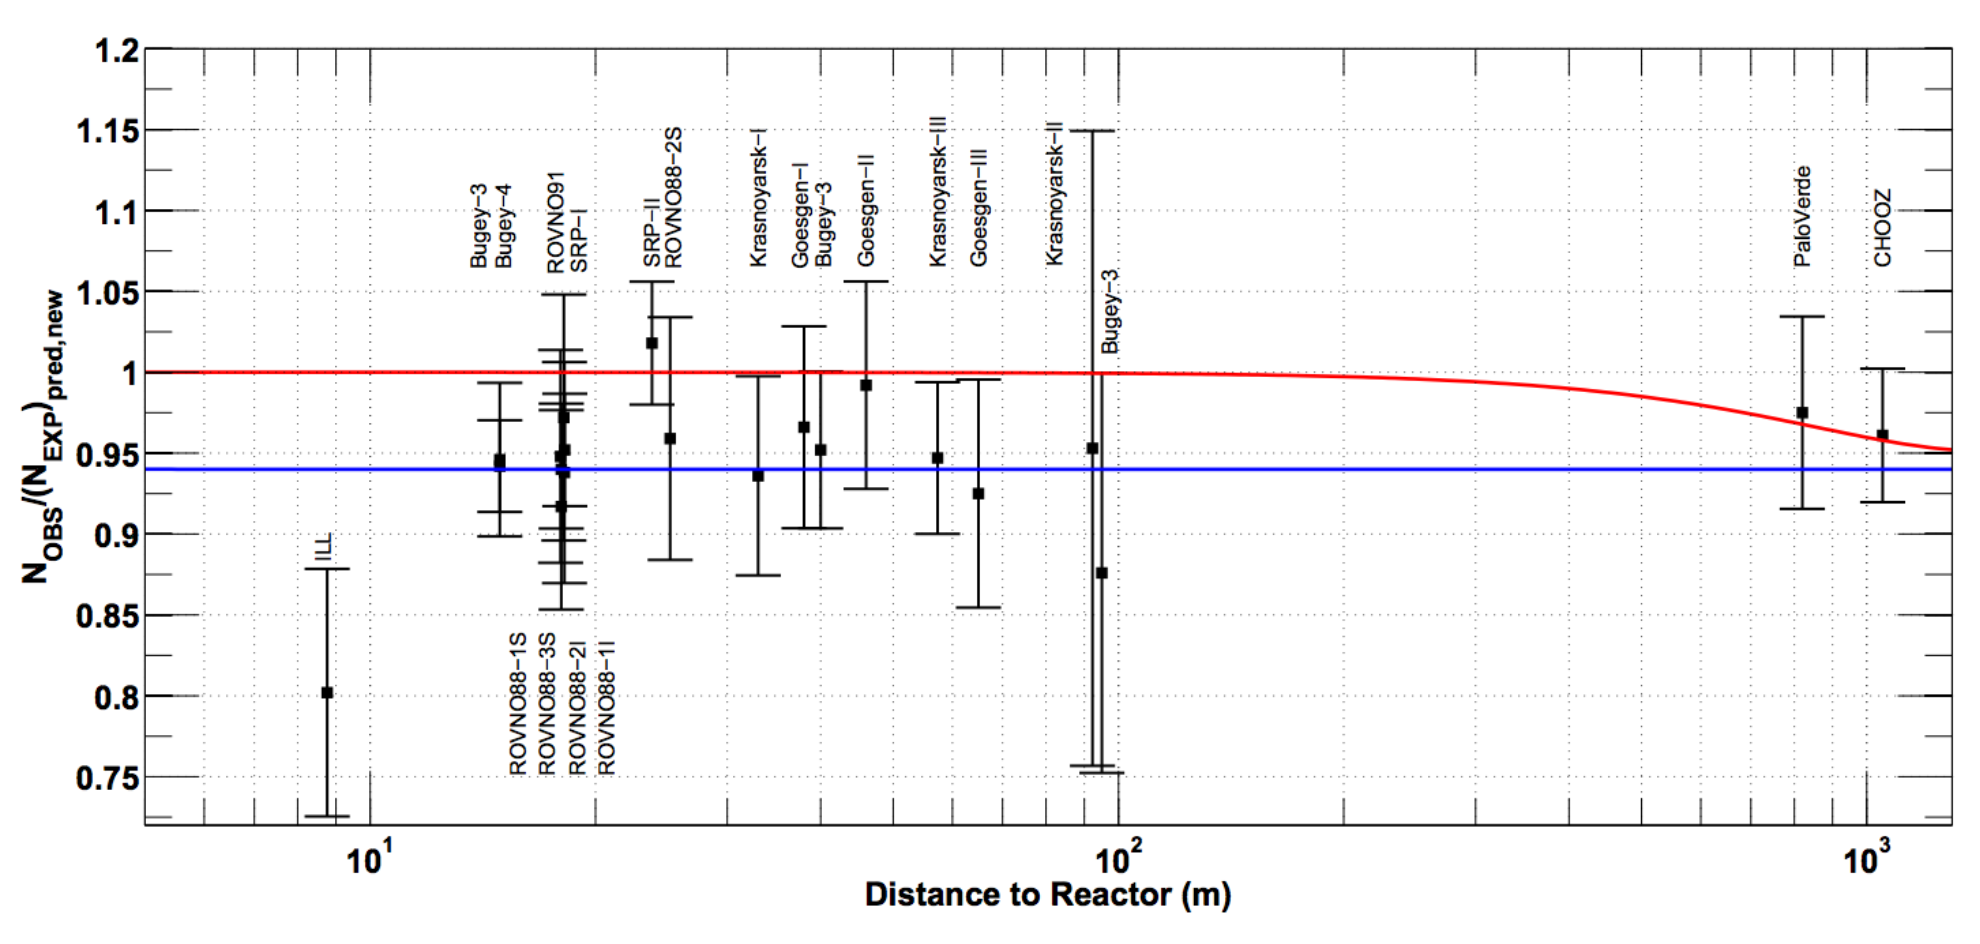
\includegraphics[width=1\columnwidth]{../figures/reactor_anom.png}
  \caption{Plot for the short baseline reactor antineutrino anomaly. The red curve shows a possible three active neutrino mixing solution, using $\sin^2\theta_{13} = 0.06$. The blue curve shows a possible solution including a new neutrino mass state with $\Delta m^2 \gg 1\text{ eV}^2$.}
\end{figure}

\section{Current and Future Experimental Efforts}
Due to the number of anomalous results to date sterile neutrino searches have become popular research topics at the majority of contemporary neutrino experiments, both those currently running and those in the design and construction phases.

\subsection{Current Experimental Results}
%matt
\subsubsection{MINOS/MINOS+}
The MINOS (Main Injector Neutrino Oscillation Search) experiment ran from 2005 to 2012 and its wide-band fresh, MINOS+, has taking data since September 2013. The MINOS experiment is a long baseline style detector with a neutrino beam source and near detector at Fermilab and a far detector located in northern Minnesota. Though its primary physics goals lie in the area of neutrino oscillation measurements, MINOS and MINOS+ are now also running sterile neutrino analysis with their data. MINOS detects sterile neutrinos via their disappearance in neutral-current (NC) interactions, which are independent of the three known neutrino flavors and their oscillations, and in charged-current (CC) interactions differing from those predicted from the mixing of the three neutrinos of the standard model. The latest sterile neutrino results from the collaboration \cite{MINOS} now exclude a large majority of the LSND allowed phase space, Figure~\ref{fig:MINOS}. These exclusion limits are predicted to increase by up to a factor of 2 as MINOS+ continues to run.

\begin{figure}[H]
  \centering
  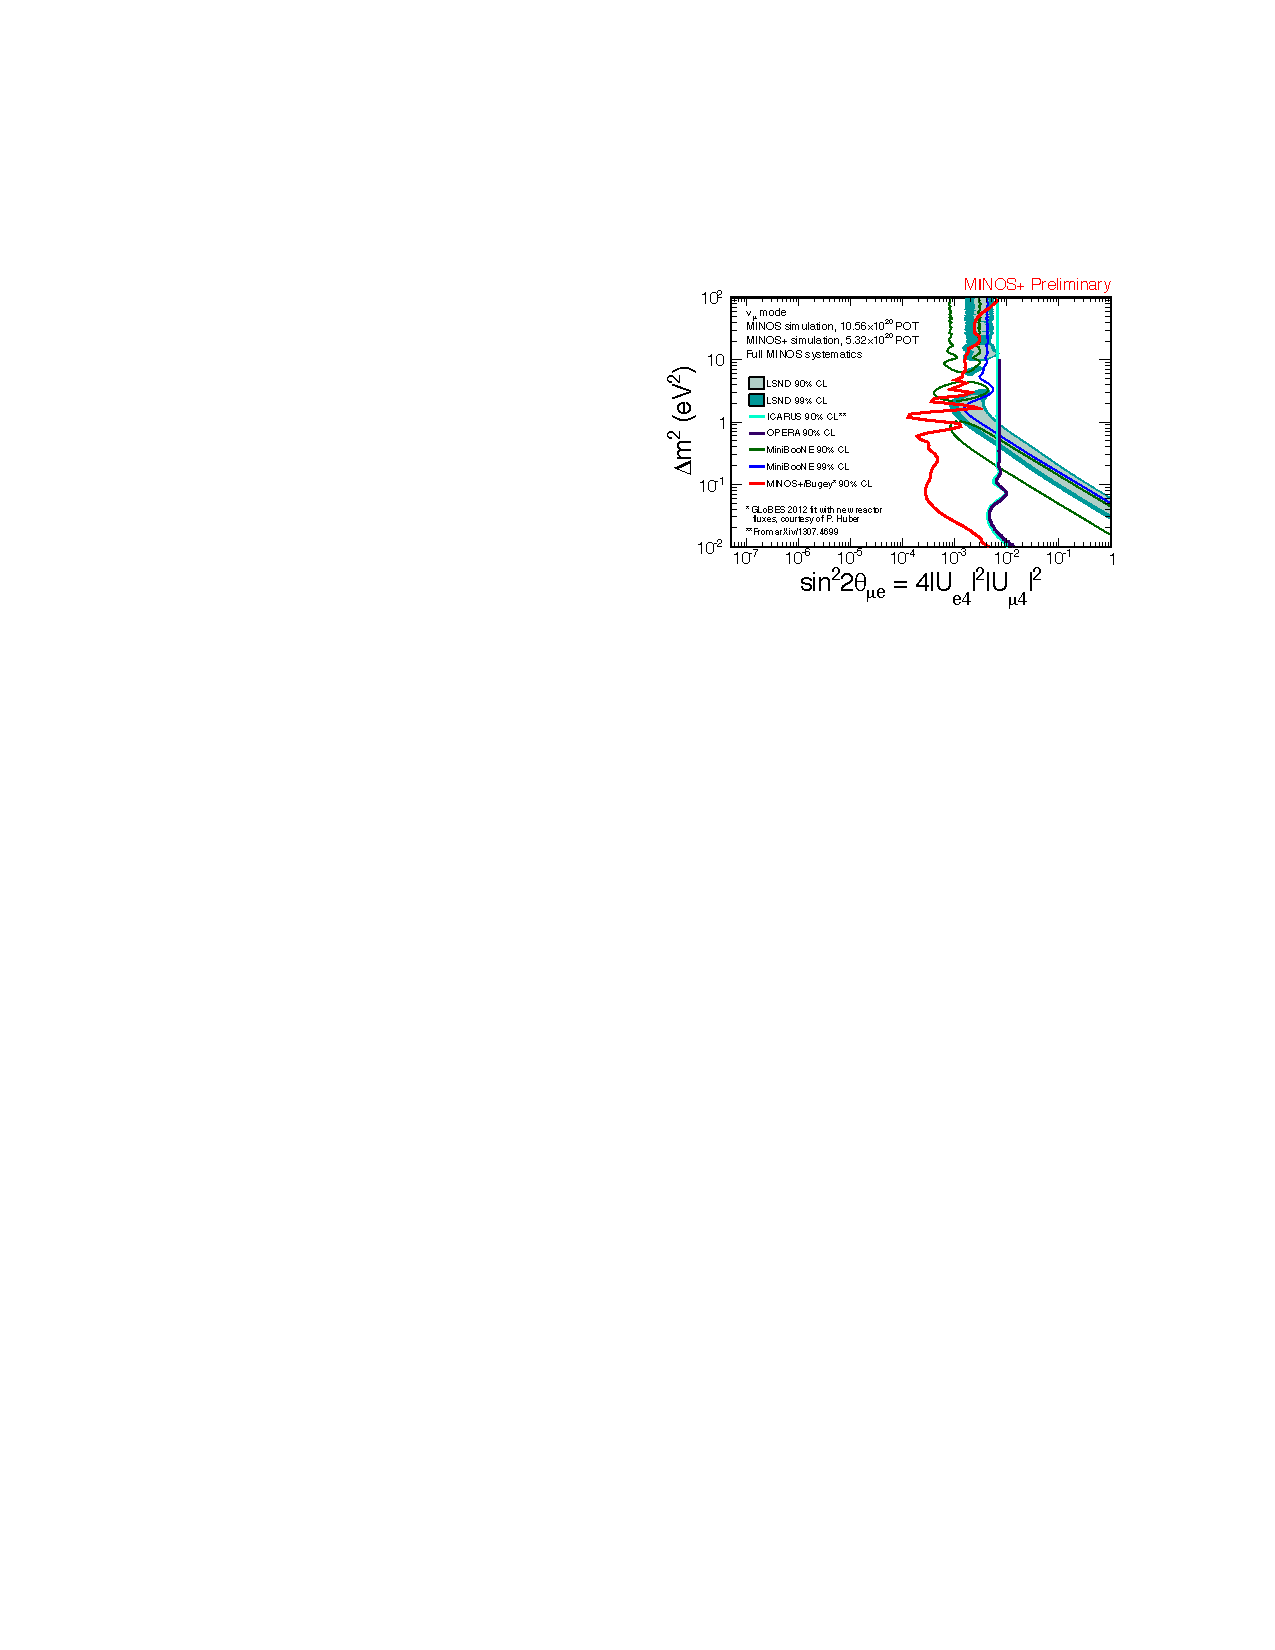
\includegraphics[width=1\columnwidth]{../figures/minos2.pdf}
  \caption{MINOS sterile neutrino exclusion limits~\cite{MINOS}. MINOS is now excluding (to the right of the red line) much of the LSND allowed phase space (shaded).}
  \label{fig:MINOS}
\end{figure}

\subsubsection{Super-Kamiokande}
The Super-Kamiokande experiment is a 22.5 kton water Cherenkov detector that looks at atmospheric neutrino oscillations. Their latest sterile neutrino analysis~\cite{SuperK} used a sterile vacuum fit to put limits on the mixing between $\nu_{\mu}$ and a sterile neutrino $\nu_4$, parameterized by $\left|U_{\mu 4}\right|^2 \approx \sin^2 \theta_{24}$, Figure~\ref{fig:SuperK}. Super-K can not measure $\Delta m^{2}_{41}$ in this analysis however, so when comparing to MiniBooNE the Super-K result is just a straight line. The Super-K result is is consistent with the MiniBooNE exclusion, providing verification on at least part of the MiniBooNE excluded region.

\begin{figure}[H]
 \centering
 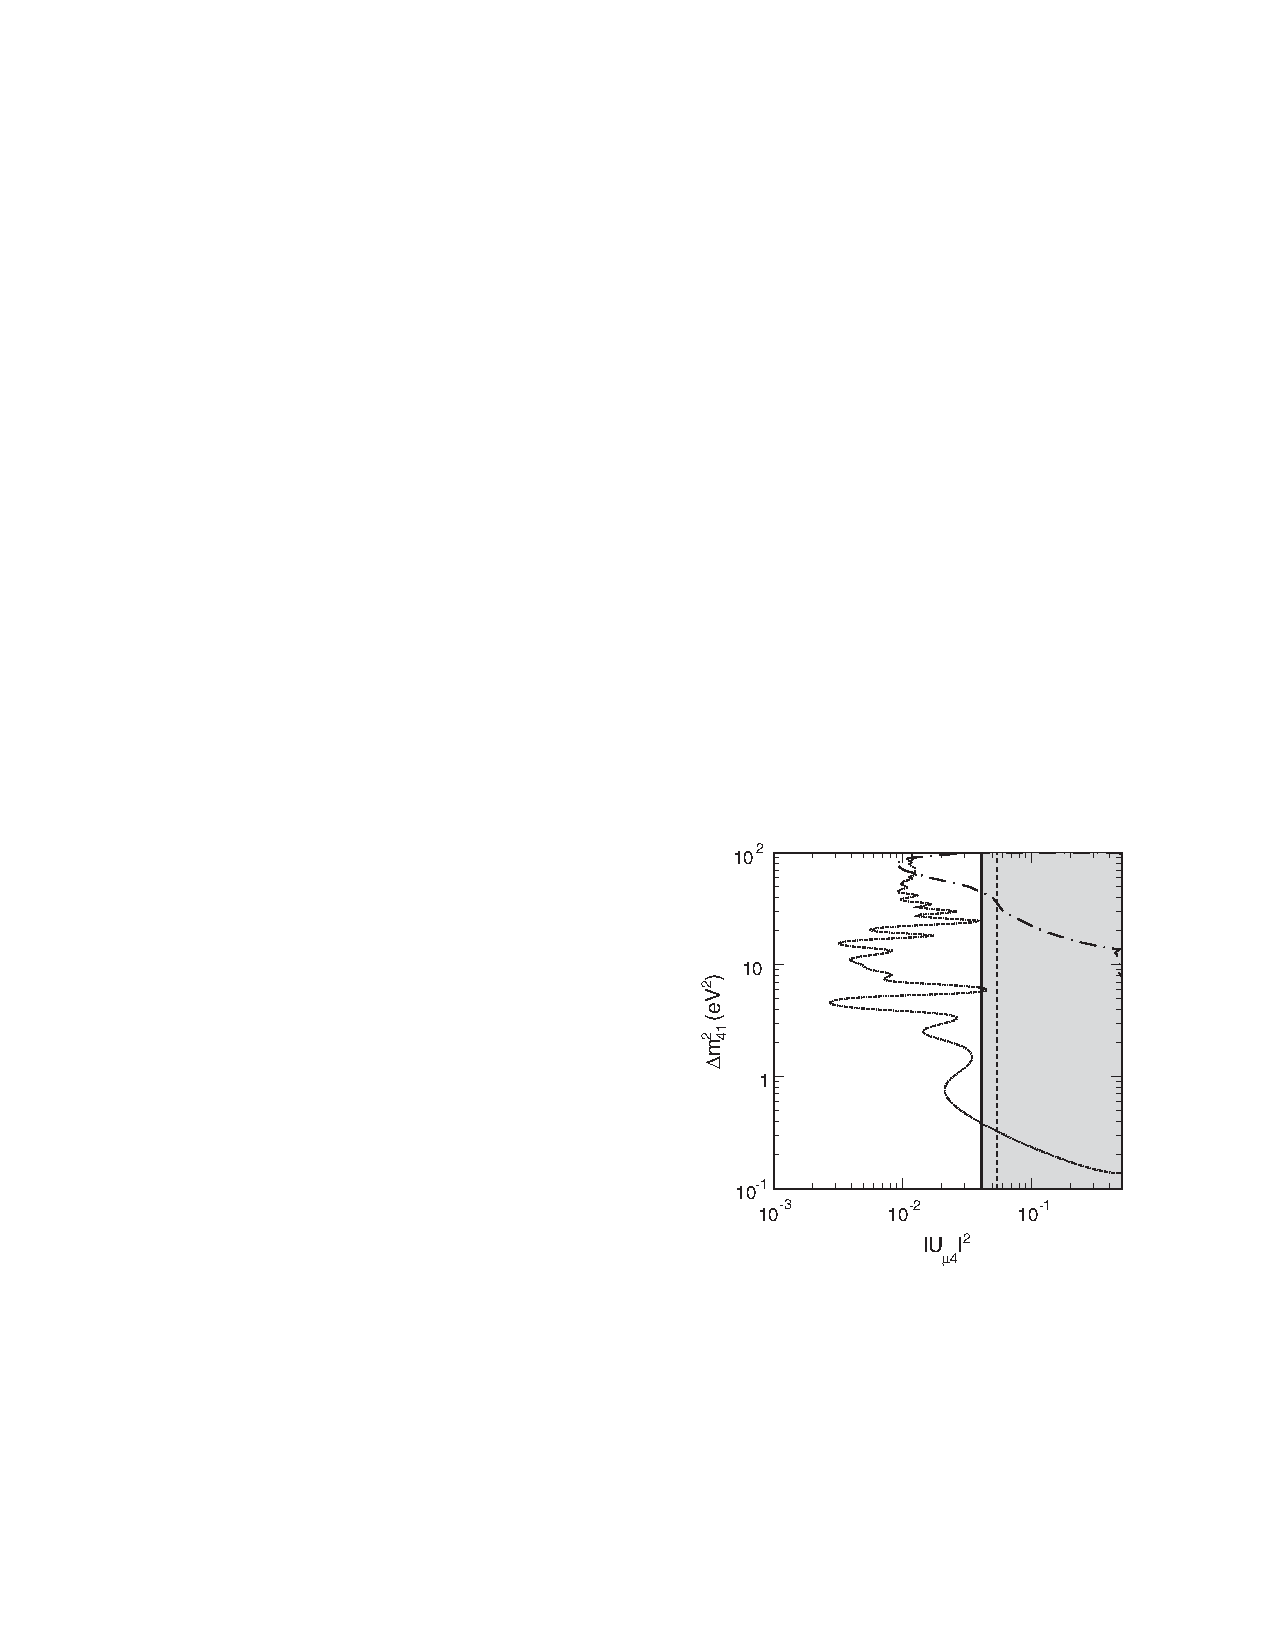
\includegraphics[width=1\columnwidth]{../figures/sk1.pdf}
 \caption{Super-Kamiokande sterile neutrino exclusion limits at 90\% (solid) and 99\% (dashed) confidence~\cite{SuperK}. The Super-K sterile vacuum fit can not measure $\Delta m^{2}_{41}$ so it is plotted as a straight line when compared to the joint analysis of MiniBooNE and SciBooNE (dotted) at 90\% confidence.}
 \label{fig:SuperK}
\end{figure}

\subsubsection{Daya Bay}
The Daya Bay experiment is a reactor antineutrino experiment with six liquid scintillator detectors located at different baselines from six 2.9 GW$_\text{th}$ nuclear reactors. It is able to make sterile neutrino measurements at smaller mass squared differences, $10^{−3} \text{ eV}^2  \lesssim \left|\Delta m^{2}_{41}\right| \lesssim 0.1 \text{ eV}^2$, than have been probed by other experiments to date~\cite{DayaBay}. While they have many different combinations of their detectors data sets, the Daya Bay exclusion limits mark out more of the small mass difference phase space than the combined LSND and KARMEN limits.

\begin{figure}[H]
  \centering
  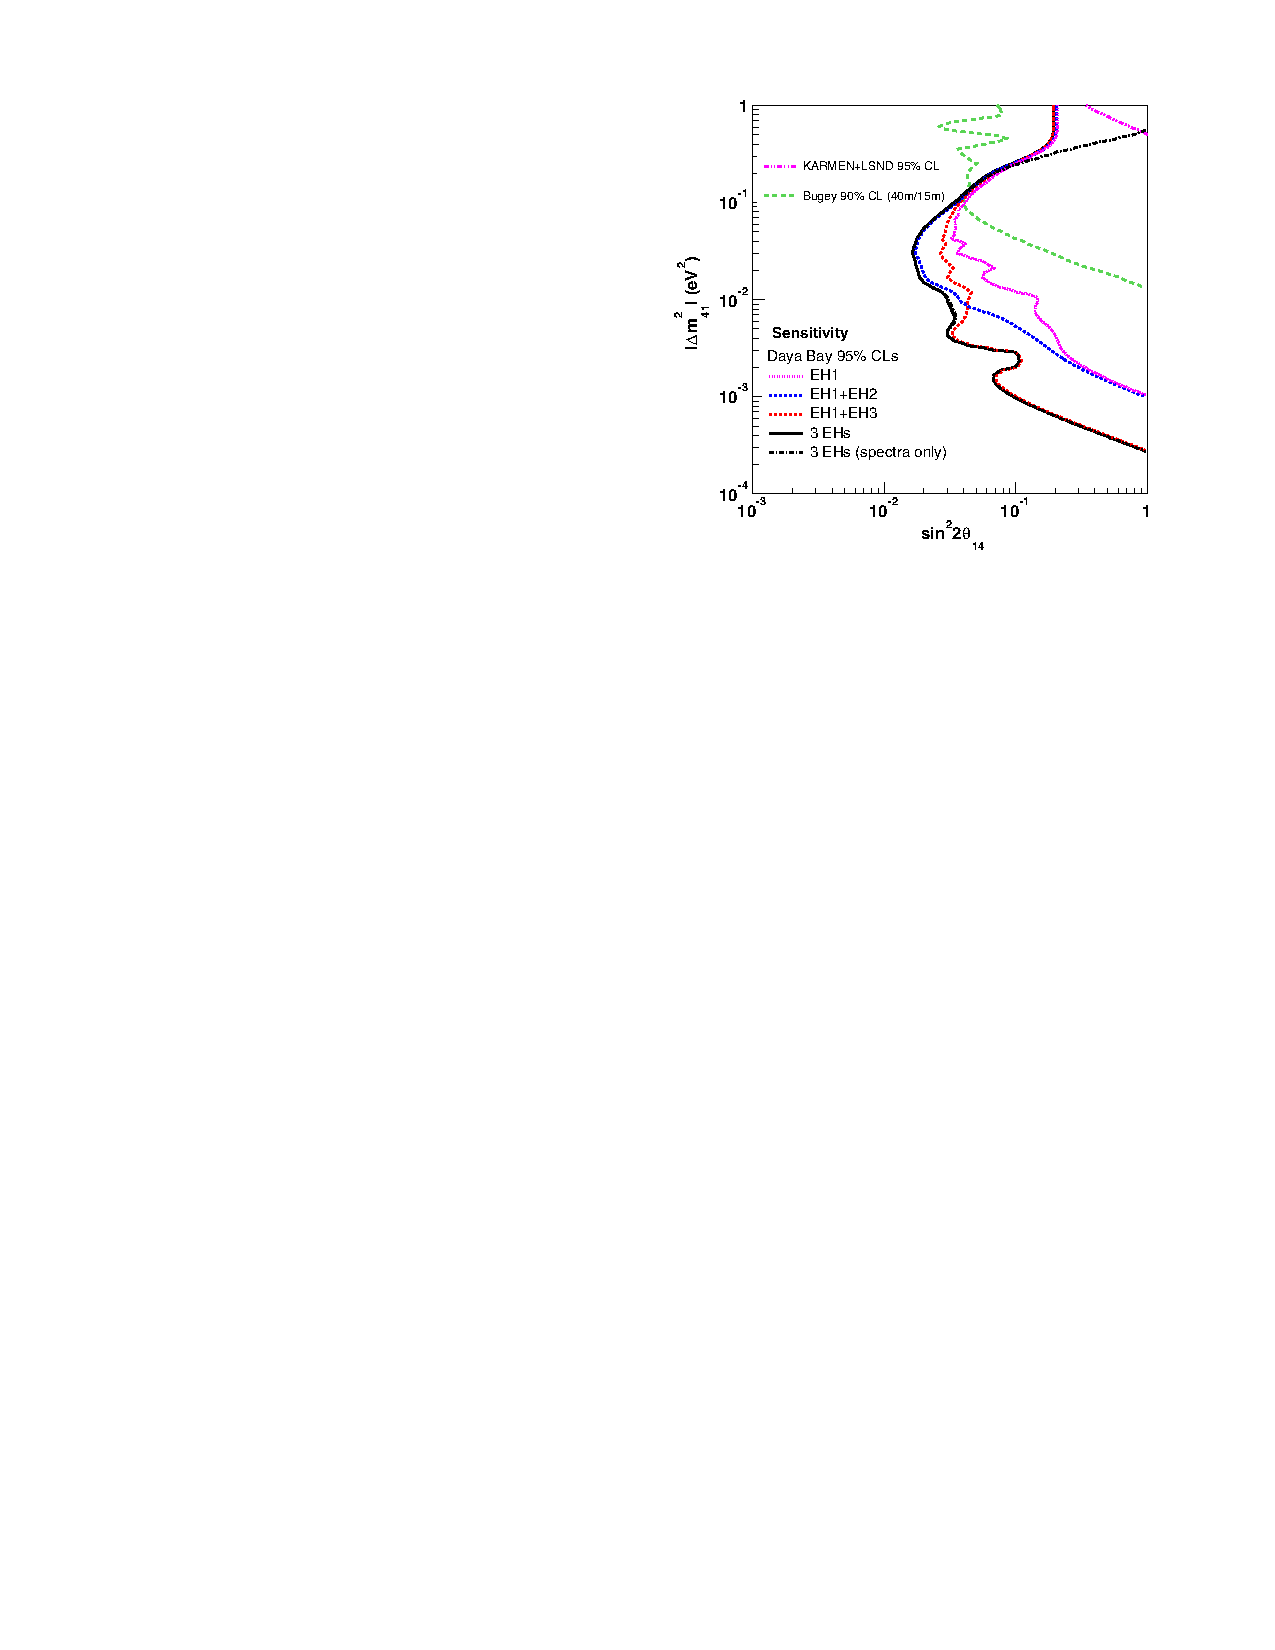
\includegraphics[width=1\columnwidth]{../figures/daya1.pdf}
  \caption{Daya Bay sterile neutrino exclusion limits~\cite{DayaBay}.}
  \label{fig:DayaBay}
\end{figure}


\subsection{Future Experiments}
% Matt
While there are many future neutrino experiments in various stages of development, MicroBooNE and NOvA are the closest to producing new sterile neutrino results. As its name suggests, MicroBooNE is the larger follow up experiment to MiniBooNE. The MicroBooNE detector is an advanced time projection chamber with a 60 ton fiducial volume of liquid argon, and unlike MiniBooNE it will be able to distinguish between photons and electrons. It is widely expected that these significant improvements will allow MicroBooNE to resolve the MiniBooNE excess anomaly. The NOvA experiment is a long baseline experiment that uses the same NuMI neutrino beam from Fermilab as MINOS and also has its far detector located in northern Minnesota. The 330 ton near and 14 kton far detectors are liquid scintillator designs located near the surface. NOvA's primary purpose is to make oscillation measurements, including potentially determining the ordering of the mass hierarchy, but will produce more sterile neutrino measurements as well.

\section{Conclusions}
The discovery of heavy, right-handed sterile neutrinos would help explain some of the mystery surrounding the nature of neutrinos.  While there is some evidence for sterile neutrinos from LSND and MiniBooNE, it is very hotly contested evidence.  Further work remains to be done before the answer is clear.  Neutrino specific experiments like MINOS+, Super-K, and Daya Bay are continuing the search for evidence for sterile neutrinos.  As the amount of data continues to increase, the anomalies will certainly be confirmed or refuted very soon.

\begin{thebibliography}{9}
\bibitem{ping1}
  T2K Experiment -- \url{http://t2k-experiment.org/neutrinos/in-the-standard-model/}
\bibitem{ping2}
Solar neutrinos. Rep. Prog. Phys. 64 (2001) 97–146
\bibitem{ping3}
Daya Bay Experiment: \url{https://www.bnl.gov/science/dayabay.php}
\bibitem{ping4}
Neutrinoless double beta decay and CP violation Physics Letters B Volume 157, Issues 5–6, 25 July 1985, Pages 442–446
\bibitem{ping5}
Neutrinoless Double Beta Decay Experiments. arXiv:1408.2455v1 [hep-ex] 11 Aug 2014

\bibitem{ponte}
  B.~Pontecorvo,
  Mesonium and antimesonium,
  \emph{Sov. Phys. JETP} {\bf 6}, 429 (1957).
\bibitem{MNS}
  Z.~Maki, M.~Nakagawa, and S.~Sakata,
  Remarks on the Unified Model of Elementary Particles,
  \emph{Progress of Theoretical Physics} {\bf 28}(5), 870–880 (1962).
\bibitem{matrixpara}
  L.~L.~Chau and W.~Y.~Keung,
  Comments on the Parametrization of the Kobayashi-Maskawa Matrix,
  \emph{Phys. Rev. Lett.}, {\bf 53}, 1802 (1984).

\bibitem{justin1}
Biswajoy Brahmachari, A see-saw model of sterile neutrino, \emph{Phys. Lett. B,}, {\bf 461} 3, 26 August 1999, Pages 243-247.
\bibitem{justin2}
W. Grimus, L. Lavoura, B. Radovcic, Type II seesaw mechanism for Higgs doublets and the scale of new physics, \emph{Phys. Lett. B.}, {\bf 674}, 2, 13 April 2009, Pages 117-121.
\bibitem{LSND}
  A.~Aguilar-Arevalo \emph{et al.} Evidence for neutrino oscillations from the observation of anti-neutrino(electron) appearance in a anti-neutrino(muon) beam. \emph{Phys. Rev. D.}, {\bf 64} 112007, 2001.
\bibitem{mini1}
  A.~Aguilar-Arevalo \emph{et al.} Event Excess in the MiniBooNE Search for $\nu_\mu \rightarrow \nu_e$ Oscillations. \emph{Phys. Rev. Lett.}, {\bf 105} 181801, 2010.
\bibitem{mini2}
  A.~Aguilar-Arevalo \emph{et al.} Improved Search $\nu_\mu \rightarrow \nu_e$ Oscillations in the MiniBooNE Experiment. \emph{Phys. Rev. Lett.}, {\bf 110} 161801, 2013.
\bibitem{reactor_anom1}
  G. Mention, M. Fechner, Th. Lasserre, Th.A. Mueller, D. Lhuillier, \emph{et al.} The Reactor Antineutrino Anomaly. \emph{Phys. Rev. D.}, {\bf 83} 073006, 2011.
\bibitem{reactor_anom2}
  Th. A. Mueller, D. Lhuillier, M. Fallot, A. Letourneau, S. Cormon, \emph{et al.} Improved Predictions of Reactor Antineutrino Spectra. \emph{Phys. Rev. C.}, {\bf 83} 054615, 2011.
\bibitem{gallex1}
  P.~Anselmann~\emph{et al.} First results from the Cr-51 neutrino source experiment with the GALLEX detector. \emph{Phys. Lett. B.}, {\bf 342} 440-450, 1995
\bibitem{gallex2}
  W.~Hampel~\emph{et al.} Final results of the Cr-51 neutrino source experiments in GALLEX. \emph{Phys. Lett. B.}, {\bf 420} 114-126, 1998.
\bibitem{sage1}
  Dzh.~N.~Abdurashitov, V.N.~Gavrin, S.V. Girin, V.V. Gorbachev, Tatiana V. Ibragimova, \emph{et al.} The Russian-American gallium experiment (SAGE) Cr neutrino source measurement. \emph{Phys. Rev. Lett.}, {\bf 77} 4708-4711, 1996.
\bibitem{sage2}
  J.~N.~Abdurashitov~\emph{et al.} Measurement of the response of the Russian-American gallium experiment to neutrinos from a Cr-51 source. \emph{Phys. Rev. C.}, {\bf 59} 2246-2263, 1999.
\bibitem{MINOS}
  Alexandre B. Sousa (for the MINOS and MINOS+ Collaborations) First MINOS+ Data and New Results from MINOS. arXiv:1502.07715v1 [hep-ex] \url{http://arxiv.org/abs/1502.07715}
\bibitem{SuperK}
  K. Abe~\emph{et al.} (Super-Kamiokande Collaboration) Limits on sterile neutrino mixing using atmospheric neutrinos in Super-Kamiokande. \emph{Phys. Rev. D}, {\bf 91}, 052019, 2015, \url{http://dx.doi.org/10.1103/PhysRevD.91.052019}
\bibitem{DayaBay}
  F. P. An~\emph{et al.} (Daya Bay Collaboration) Search for a Light Sterile Neutrino at Daya Bay. \emph{Phys. Rev. Lett.} {\bf 113}, 141802, 2014, \url{http://dx.doi.org/10.1103/PhysRevLett.113.141802}

\end{thebibliography}

\end{document} %%% end of doc %%%
